\documentclass[sigconf,natbib=true,anonymous=true]{acmart}

\settopmatter{printacmref=true}
\acmConference[CHIIR '27]{2027 ACM SIGIR Conference on Human Information Interaction and Retrieval}{March 7--11, 2027}{Berlin, Germany}
\acmYear{2027}
\copyrightyear{2027}
\acmISBN{}
\acmDOI{}

\title{More Citations or More Sources? Source Breadth in Human Preferences for Generative Search}

\begin{document}

\begin{abstract}
Generative search systems do not only answer questions; they also curate a visible evidence surface through the sources they cite. Existing human-preference analyses largely measure citation abundance or source type, leaving open whether breadth across domains is a valid user-centered signal beyond the number of citations. Using Search Arena's public paired-comparison logs, we conduct a frozen, outcome-blind confirmatory analysis of 4,265 decisive, English, first-turn battles. We resolve user-visible citations to canonical URLs and registrable domains, define same-domain redundancy as citation quantity minus unique-domain count, and fit a contextual Bradley--Terry model controlling model strength, response length, source categories, and citation presentation. The standardized redundancy coefficient was 0.028 (odds ratio 1.028; judge-cluster bootstrap 95\% CI $[-0.071,0.127]$; $p=.576$), and adding redundancy produced no reliable held-out gain in log loss or Brier score. In 173 battles with equal citation counts but different breadth, the broader-sourced response won 57.2\% of votes (95\% CI 49.7--64.8\%; descriptive $p=.068$), a suggestive but imprecise pattern. The omnibus intent interaction was significant, but no intent-specific effect survived Holm correction, and exact model-pair estimates disagreed in sign. Across construct separation, incremental prediction, and transportability checks, breadth is measurable but does not behave as a stable, portable preference metric in this dataset. For preference-oriented evaluation, citation quantity and domain breadth should therefore be treated as distinct dimensions rather than collapsed into a single citation-richness signal.
\end{abstract}

\ccsdesc[500]{Information systems~Users and interactive retrieval}
\ccsdesc[300]{Information systems~Search interfaces}
\ccsdesc[300]{Human-centered computing~Human computer interaction (HCI)}
\keywords{generative search, human information interaction, citations, source breadth, user preference, information retrieval}

\maketitle

\section{Introduction}
Generative search systems increasingly mediate access to web information by retrieving sources and synthesizing them into a single conversational response. Traditional web search exposes a ranked set of documents and asks the searcher to decide what to inspect and combine; generative search performs part of that selection and synthesis upstream, then exposes only a subset of sources through citations and reference links. The resulting answer is therefore not only a textual summary but also a designed surface of evidence.

Prior work shows that this evidence surface matters. Search Arena, a large-scale in-the-wild evaluation of search-augmented language models, found that human preferences are associated with response length, citation quantity, and some source categories \citep{miroyan2026searcharena}. CHIIR studies likewise show that people blend search and chat partly on the basis of trust and convenience \citep{mayerhofer2025blending}, that verification of LLM outputs is often difficult \citep{scozzi2026infallible}, and that changing how sources are presented can alter attention and downstream judgments even when source clicking remains limited \citep{he2026transparency}. Other work documents substantial provider-level differences in retrieval footprints, source diversity, citation behavior, and the gap between pages retrieved and pages exposed to users \citep{kirsten2026characterizing,strauss2026attribution,huang2026answerbubbles}. These findings establish that sourcing structure is neither uniform across systems nor a neutral detail of the interface.

Yet citation \emph{quantity} and source \emph{breadth} are distinct. An answer with eight citations may cite eight different domains, or eight pages drawn from only one or two domains. Both answers have the same citation count, but they expose users to structurally different source sets. Treating both as ``eight citations'' collapses citation abundance and repeated sourcing from already represented domains.

This creates a measurement-validity problem for user-centered evaluation. Citation count can increase without expanding the set of represented sources, while a unique-domain count can increase without establishing that the added domains provide independent evidence, different viewpoints, or a better user experience. A benchmark that rewards both citation count and unique-domain count can therefore encode two distinct preference assumptions under a single notion of ``citation richness.'' Whether the second assumption adds user-centered value beyond the first is not automatic; it must be tested. Our empirical object is therefore not a new diversity score but a concrete evaluation decision: once citation count is already represented, should breadth receive additional credit as a preference-oriented signal?

This distinction is timely because citation quantity and diversity need not move preference in the same direction. In scientific question answering, \citet{hou2026citations} found that human judges preferred more diverse citations while preferring fewer citations overall. Scientific QA, however, is a comparatively narrow source and task environment. In-the-wild generative web search spans factual lookup, synthesis, recommendation, analysis, guidance, and other information needs. Whether source breadth provides information about preference beyond citation count in this broader setting remains unresolved.

There are also plausible mechanisms in competing directions. A broader source set could offer more verification routes, signal corroboration, or expose the user to a wider evidence base. Conversely, a concentrated source set may appear more coherent or authoritative, may reduce inspection cost, or may simply be easier to process. A third possibility is that breadth has little direct effect because users often do not inspect citations closely enough for domain composition to influence preference. Recent CHIIR work on trust, verification, and citation visibility makes all three possibilities plausible \citep{mayerhofer2025blending,bink2026canyoutellme,he2026transparency}. We therefore treat breadth as an empirical property of information exposure rather than presuming that ``more domains'' is normatively or behaviorally better.

We ask a deliberately narrow empirical question: after accounting for how many citations an answer presents and for other measured response characteristics, is the breadth of represented domains associated with which answer people prefer? This is an evaluation question rather than a cognitive-mechanism claim. We do not assume that distinct domains represent distinct viewpoints, independent evidence, or higher factual quality, and we do not assume that users consciously inspect source diversity.

We study this question using Search Arena's public logs of paired comparisons. We distinguish the number of user-visible cited URLs from the number of registrable domains represented by those URLs and define same-domain redundancy as the number of citation slots that repeat an already represented domain. Our outcome-blind confirmatory design combines contextual Bradley--Terry models with exact citation-count comparisons, source-category controls, judge-clustered uncertainty, exact model-pair analyses, and pre-specified robustness checks.

The paper asks three research questions:
\begin{itemize}
    \item \textbf{RQ1:} Holding citation quantity and measured response characteristics constant, how is same-domain redundancy associated with human preference?
    \item \textbf{RQ2:} Does domain breadth add held-out predictive information beyond model identity, response length, citation quantity, citation presentation, and source category?
    \item \textbf{RQ3:} Does the quantity--breadth relationship vary across information-seeking intents?
\end{itemize}

Our contribution is deliberately narrower than a claim that source diversity is universally beneficial. First, we provide a reproducible operational separation between citation abundance and registrable-domain breadth in the sources that users can actually see. Second, we test whether breadth adds explanatory and held-out predictive information about preference once citation quantity and established response-level correlates are represented. Third, we test whether that relationship is stable enough across tasks, model pairs, and measurement choices to support a general ``more domains is better'' rule. The established positive association for citation quantity does not extend automatically to breadth: the pooled term is near zero, held-out prediction does not improve, and localized estimates are not stable enough to justify a portable bonus for breadth. Our novelty lies in this validation question and its in-the-wild transport tests, not in claiming that domain counts themselves are new.

\section{Related Work}
\subsection{Generative search and human preference}
Search-augmented language models combine web retrieval with generated synthesis, producing an answer-first interface rather than a ranked list of independent documents. Search Arena provides the closest empirical foundation for the present study: it contains paired, in-the-wild interactions with search-augmented systems and shows that users tend to prefer longer answers, answers with more citations, and answers citing some source categories such as community or coding sources \citep{miroyan2026searcharena}. Complementary CHIIR work shows that users switch between search and chat based partly on trust, confidence, and ease of use \citep{mayerhofer2025blending}, reinforcing that interface-level evidence cues can matter even when users do not evaluate them perfectly. Existing preference analyses, however, treat citation quantity and source type as response features; they do not isolate whether the \emph{distribution} of a fixed number of citations across domains contributes additional preference information.

Recent work also shows that generative-search systems expose materially different source environments. \citet{kirsten2026characterizing} report substantial variation across engines in external-knowledge use, source diversity, retrieval footprints, and stability. \citet{huang2026answerbubbles} characterize differences in information exposure across AI-mediated search systems, while \citet{allaham2026syntheticsources} audit citation-source composition and evidence of AI-generated sources. These studies motivate source breadth as an evaluation target but are primarily system audits rather than analyses of pairwise human preference.

\subsection{Citations, attribution, and verification}
Citations in generated answers function both as routes to verification and as visible signals about the evidential basis of an answer. Those functions need not align. Search Arena reports that human preferences respond positively to citation count even when citation support is imperfect \citep{miroyan2026searcharena}. Using LMArena search logs, \citet{strauss2026attribution} document provider-level differences in the gap between search results visited and sources ultimately cited. In CHIIR, \citet{scozzi2026infallible} show that researchers face substantial challenges verifying LLM outputs, while \citet{bink2026canyoutellme} show that an intervention can prompt reflection without straightforward gains in correctness or search engagement. \citet{he2026transparency} further show that citation presentation changes source attention and downstream outcomes, while actual source clicking remains limited. Together, this literature cautions against equating citation visibility with factual quality and suggests that sourcing can operate both as actionable evidence and as a surface-level interface cue.

Our outcome is therefore not citation correctness, successful verification, or source inspection. We study the structure of the \emph{user-visible} citation set and its association with comparative preference.

\subsection{Citation quantity, breadth, and information exposure}
Citation diversity can refer to URLs, registrable domains, publishers, ownership groups, source categories, topical aspects, or viewpoints. The broader information-retrieval literature treats diversification partly as an exposure and coverage problem, with diversified result sets capable of altering source exposure, aspect coverage, and search behavior \citep{nikolov2019exposure,maxwell2019diversification}. Recent generative-search work likewise distinguishes citation breadth from citation intensity when auditing marketplace exposure \citep{cheng2026citationgovernance}. That work concerns system-level exposure rather than comparative human preference, but it reinforces that abundance and breadth are analytically distinct. We adopt a deliberately conservative operationalization: registrable-domain breadth. Different domains may share ownership, reproduce the same reporting, or express the same perspective; our measure therefore does not imply viewpoint diversity or evidence independence.

The closest preference study is \citet{hou2026citations}, who examine citation features in scientific-QA pairwise preference data and find separable relationships for citation quantity and diversity. Search Arena establishes preference associations for citation quantity and source type in heterogeneous web search \citep{miroyan2026searcharena}; Cheng separates breadth from intensity for system-level e-commerce exposure \citep{cheng2026citationgovernance}; Hou connects citation diversity to preference in scientific QA. The unresolved intersection is whether breadth contributes \emph{incremental} preference information in heterogeneous, in-the-wild generative web search and whether that relationship transports across systems and tasks. That is the question tested here.

\subsection{From source features to evaluation metrics}
Measurement-theoretic work on model evaluation distinguishes a feature that can be computed from one that validly supports an intended inference \citep{xiao2023metricleval}. We do not propose a new general theory of metric validity. Instead, we apply that principle to one concrete generative-search decision: whether domain breadth should receive additional credit as a preference-oriented signal once citation abundance is already represented. We use three tests (Table~\ref{tab:validity}). \emph{Construct separation} asks whether breadth captures visible sourcing structure not reducible to citation abundance. \emph{Incremental preference validity} asks whether breadth explains or predicts preference beyond abundance and established response-level correlates. \emph{Transportability} asks whether any relationship is stable enough across tasks, systems, and reasonable measurement choices to support a general evaluation rule. These tests are deliberately outcome-specific: breadth may still be useful for coverage or auditability even if it is not useful for predicting human preference.

User-visible source structure may matter through corroboration, verification opportunity, interface signaling, or not at all if source attention is low. These competing mechanisms make a directional breadth hypothesis difficult to justify across heterogeneous tasks and models. We therefore use intent and exact model-pair analyses as transportability tests rather than as opportunities to search for a preferred subgroup result.

\begin{table}[t]
\centering
\caption{Decision tests for treating source breadth as a preference-oriented evaluation signal.}
\label{tab:validity}
\small
\begin{tabular}{p{0.31\columnwidth}p{0.61\columnwidth}}
\toprule
Decision question & Evidence used here \\
\midrule
Distinct from abundance? & Separate $C$, $U$, and $R$; inspect identification; exact-count comparison \\
Adds preference signal? & M3$\rightarrow$M4 fit, effect magnitude, and judge-grouped held-out prediction \\
Portable across settings? & Intent interactions, exact model pairs, and prespecified measurement sensitivities \\
\bottomrule
\end{tabular}
\end{table}

\section{Data, Measures, and Ethics}
\subsection{Search Arena and primary sample}
We use the public Search Arena 24K release of paired interactions with search-augmented language models \citep{miroyan2026searcharena}. The confirmatory unit is a paired battle in which two systems answer the same user interaction and a human preference judgment is recorded. The primary sample is restricted to first-turn, English-language, decisive votes among eligible search-augmented models. Released automated intent labels do not determine primary-sample inclusion and are used only in secondary heterogeneity analyses. We impose no minimum citation-count threshold, retaining responses with zero or one measurable visible citation to avoid conditioning on provider-specific citation behavior.

\begin{table}[t]
\centering
\caption{Primary-sample construction. Restrictions were frozen before source-breadth preference coefficients were estimated.}
\label{tab:funnel}
\small
\begin{tabular}{lr}
\toprule
Stage & Remaining records \\
\midrule
All feature rows & 24,069 \\
Recorded preference vote & 12,652 \\
Decisive vote & 8,613 \\
First turn & 6,899 \\
English & 4,440 \\
Eligible search models & 4,265 \\
\bottomrule
\end{tabular}
\end{table}

This study is a secondary analysis of a public, anonymized research dataset: we recruited no new participants and collected no new personal data. We analyze only fields released for research, make no attempt to identify users, and use anonymized judge identifiers only to account for repeated judgments when estimating uncertainty.

\subsection{User-visible citation resolution}
Numeric citation markers are resolved through the corresponding disclosed search trace. Direct Markdown links, autolinks, and bare HTTP(S) URLs are treated as user-visible sources even when absent from a provider's disclosed trace; a disclosed trace is therefore not itself an inclusion requirement. Trace grounding is retained as a diagnostic and robustness variable. URLs are canonicalized before deduplication and mapped to registrable domains with a Public Suffix List implementation. This format-invariant rule was frozen before preference modeling because providers expose citations through different visible syntaxes and trace completeness differs across systems.

\subsection{Citation quantity and source breadth}
For each response, let $C$ denote the number of distinct canonical user-visible source URLs and $U$ the number of unique registrable domains. The primary redundancy measure is
\begin{equation}
R = C-U.
\end{equation}
At fixed $C$, larger $R$ indicates greater repetition of already represented domains. Because $R=C-U$, the terms $\beta_C C + \beta_R R$ can be rewritten as $(\beta_C+\beta_R)C-\beta_R U$. The $(C,R)$ parameterization is therefore algebraically equivalent to modeling citation quantity and unique-domain count directly; it is chosen because repeated-domain citation slots have an immediate interpretation. Conditional on citation quantity, $-\beta_R$ is exactly the coefficient corresponding to one additional represented domain. \textbf{Thus, a positive $\beta_R$ means less breadth is associated with preference, whereas a negative $\beta_R$ means broader sourcing is associated with preference.} We report conditioning diagnostics plus an exact citation-count comparison to assess empirical identification rather than relying on the parameterization alone.

\begin{table}[t]
\centering
\caption{Illustration of equal citation quantity but different domain breadth.}
\label{tab:construct}
\small
\begin{tabular}{lrrr}
\toprule
Visible sources & $C$ & $U$ & $R$ \\
\midrule
Six URLs from six domains & 6 & 6 & 0 \\
Six URLs from two domains & 6 & 2 & 4 \\
\bottomrule
\end{tabular}
\end{table}

A benchmark that automatically rewards larger $U$ would rank the first row above the second despite identical citation quantity. That ranking may be appropriate for a coverage-oriented objective, but it becomes a user-preference claim only if broader sourcing is actually associated with the user outcome of interest. The analyses below test that narrower claim.

\subsection{Covariates}
We measure response length, model identity, citation presentation where released, and deterministic source-category counts following the Search Arena taxonomy: YouTube, government/education, wiki, U.S. news, foreign news, social media, community/blog, technical/coding, academic journal, retail, and other. The \textit{other} source category serves as the reference category. Released primary-intent labels enter only secondary heterogeneity analyses. For robustness, we retain the public timestamp as ISO calendar week and extract client country only when both response-side metadata records agree.

\section{Analysis}
\subsection{Outcome-blind feasibility and reproducibility}
Before fitting any preference model, we audited sample size, measurable citation variation, parsing coverage, design rank, conditioning, connectedness of the model-comparison graph, and within-model-pair redundancy variation without examining the relationship between breadth and preference. The audit was a feasibility gate, not an outcome-selection procedure: it could stop the confirmatory run if the construct was not identifiable, but it could not choose among favorable effect specifications. The audit returned GREEN. The frozen plan and exact feature file were SHA-256 bound, and the confirmatory run used fixed seed 20261006. The run log records 1,000/1,000 successful primary bootstrap replicates and no post-hoc specification selected by outcome. Missing judge identifiers, where present, are treated as row-specific singleton clusters rather than dropped.

The judge-cluster bootstrap resamples judge clusters while retaining all battles belonging to each sampled judge. Judge is the natural repeated-observation unit here: after restricting to first turn, each retained conversation contributes at most one battle, while a judge may contribute multiple conversations. For held-out validation, all observations from a judge remain in the same fold and continuous predictors are standardized using training-fold statistics only. The release does not provide a validated semantic query-family identifier, so semantically similar prompts entered by different judges cannot be grouped as a common stimulus; we return to this residual dependence limitation in Section~7. For reproducibility, the frozen analysis plan, environment and hash log, feasibility report, result tables, and plotted outputs were retained in an anonymous audit bundle.

As a non-gating pipeline validity check, we re-estimated the positive preference associations for response length and citation quantity reported by Search Arena \citep{miroyan2026searcharena}. Directional disagreement would have been treated as a diagnostic warning, not as permission to alter the breadth hypothesis.

\subsection{Primary contextual Bradley--Terry model}
For each battle, response-level predictors are represented as A-minus-B differences. With $Y=1$ when A wins and $Y=0$ when B wins, the primary model is
\begin{align}
\mathrm{logit}\,P(Y=1) ={}& \alpha + (\theta_A-\theta_B) \\
&+ \beta_C\Delta C + \beta_R\Delta R + \beta_L\Delta L \\
&+ \sum_k \gamma_k\Delta S_k + \beta_F\Delta F.
\end{align}
The $\theta$ terms are Bradley--Terry model-strength parameters; $\alpha$ captures any residual A/B presentation-side preference; $\Delta L$ is response-length difference; $\Delta S_k$ are source-category differences; and $\Delta F$ captures citation presentation. Continuous differences are standardized. The primary estimand is $\beta_R$, interpreted with the sign convention defined above. Because breadth is naturally occurring rather than randomized, $\beta_R$ is a conditional association parameter, not the causal effect of adding or removing a domain. We report judge-cluster-robust uncertainty, a judge-cluster bootstrap interval, standardized and raw-unit odds ratios, and a model-implied probability contrast. RQ2 is assessed with five judge-grouped out-of-sample folds comparing the otherwise identical model with and without redundancy using held-out log loss and Brier score.

The nested specification sequence was: M0 model strength only; M1 adds response length; M2 adds citation quantity; M3 adds source-category composition; and M4 adds domain redundancy.

\begin{table}[t]
\centering
\caption{Nested model comparison on the primary sample ($N=4{,}265$). LR tests compare each model with the preceding row.}
\label{tab:nested}
\small
\begin{tabular}{lrrr}
\toprule
Model & AIC & Pseudo-$R^2$ & LR $p$ \\
\midrule
M0 & 5370.70 & 0.0000 & -- \\
M1: + length & 5193.54 & 0.0339 & $<.001$ \\
M2: + citation quantity & 5114.55 & 0.0490 & $<.001$ \\
M3: + source categories & 5114.50 & 0.0528 & .029 \\
M4: + redundancy & 5116.21 & 0.0528 & .588 \\
\bottomrule
\end{tabular}
\end{table}

\subsection{Exact-count, intent, and robustness analyses}
We separately analyze battles where $C_A=C_B$ but $R_A\ne R_B$. In this subset, citation quantity is identical by construction. We report the proportion won by the broader-sourced response with a judge-cluster-bootstrap confidence interval and descriptive binomial test.

We evaluate intent interactions first with a single omnibus likelihood ratio test and Holm-correct the intent-specific coefficients. Both reduced and full intent models include model-by-intent nuisance terms so task-specific model strength is not absorbed into citation-feature interactions. Exact model-pair analyses are limited to pre-specified major pairs with at least 100 usable battles and at least 20 nonzero redundancy contrasts. Prespecified sensitivities cover language, conversation depth, alternative breadth measures, stricter URL identity, trace-grounded citations, conservative bare-URL handling, complete marker resolution, source-category ablation, standardized citation formatting, and ties. Additional checks allow model strength to vary by calendar week and client country and give each judge equal total weight. The planned attribution-quality sensitivity uses only released Search Arena attribution labels and performs no new LLM judging.

\subsection{AI-assisted research tools}
OpenAI ChatGPT assisted with stress-testing the methodology, drafting and debugging analysis code, and organizing literature. The frozen plan specified the inclusion criteria, estimands, models, and interpretation boundaries before the source-breadth preference results were inspected. No LLM generated or altered observed data, citation annotations, participant preferences, or evaluation labels, and no LLM served as a judge. Responsibility for the analysis and manuscript remains with the human author(s).

\section{Results}
\subsection{Sample and measurement diagnostics}
The outcome-blind feasibility audit returned GREEN before any source-breadth preference coefficient was inspected. Of the 4,265 primary battles, 2,057 had a nonzero A--B redundancy contrast. The exact citation-count subset contained 712 battles, of which 173 differed in domain breadth. The model-comparison graph was connected, the M4 design was full rank (26/26), the standardized design condition number was 14.53, and $\mathrm{corr}(\Delta C,\Delta R)=0.612$. Mean measurable-reference resolution coverage exceeded 95\% in every major model family, with an overall mean of 98.5\%. This is a coverage diagnostic---the fraction of candidate visible references that can be mapped to canonical URLs---rather than a manual accuracy estimate for every parsed citation.

The pre-specified positive controls also behaved as expected. Response-length difference had a positive coefficient ($\beta=0.488$, 95\% CI [0.375, 0.601]) and citation-quantity difference had a positive coefficient ($\beta=0.410$, 95\% CI [0.310, 0.511]), replicating the previously reported directions.

\subsection{RQ1: Overall association with preference}
The primary M4 estimate for standardized domain redundancy was $\beta_R=0.028$. The corresponding standardized odds ratio was 1.028, with a judge-cluster bootstrap 95\% CI for the coefficient of $[-0.071,0.127]$ (1,000 successful replicates) and $p=.576$. The odds-ratio interval was 0.931--1.136. Because positive redundancy means less breadth at fixed citation quantity, the point estimate very slightly favors repeated-domain sourcing, but the interval is compatible with modest associations in either direction and does not support a clear overall breadth effect (Figure~\ref{fig:primary}).

\begin{figure}[t]
\centering
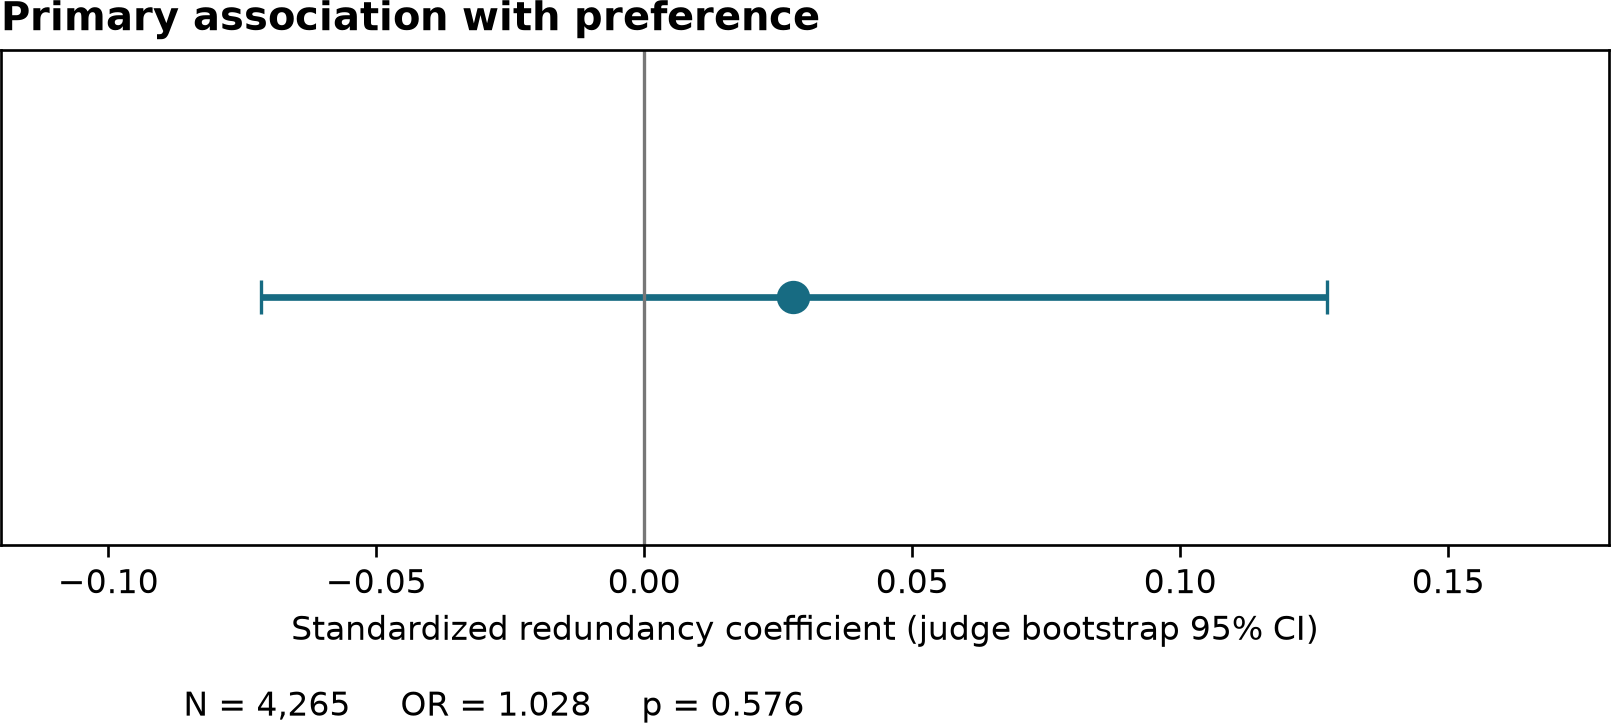
\includegraphics[width=\columnwidth]{figures/main_effect.png}
\caption{Primary association between standardized domain redundancy and preference. The horizontal interval is the judge-cluster bootstrap 95\% CI; zero denotes no association. Positive coefficients favor repeated-domain sourcing (less breadth at fixed citation quantity), and negative coefficients favor broader sourcing.}
\Description{Forest-style plot showing a standardized domain redundancy coefficient near zero, approximately 0.028, with a 95 percent confidence interval extending from about -0.071 to 0.127. The interval crosses zero.}
\label{fig:primary}
\end{figure}

The practical magnitude was also small. One additional redundant cited URL corresponded to an estimated odds ratio of 1.017. At zeroed covariate contrasts and baseline model terms, moving redundancy upward by one standard deviation shifted model-implied win probability from 48.76\% to 49.45\%, a difference of 0.69 percentage points. Mapping the bootstrap coefficient interval through the same reference configuration corresponds to shifts of approximately $-1.78$ to $+3.19$ percentage points per standard deviation. This transformation constrains the range of a uniform pooled association but is not an equivalence test: no equivalence margin was pre-specified, so we do not claim that the true effect is practically zero. Adding redundancy to M3 did not improve nested-model fit: $LR(1)=0.29$, $p=.588$, and AIC increased from 5114.50 to 5116.21.

\begin{table}[t]
\centering
\caption{Primary and complementary estimates. Primary and exact-count intervals use judge-cluster bootstrap uncertainty.}
\label{tab:main}
\small
\begin{tabular}{p{0.43\columnwidth}p{0.49\columnwidth}}
\toprule
Quantity & Estimate \\
\midrule
Primary redundancy & $\beta=0.028$; OR=1.028; 95\% CI $[-0.071,0.127]$; $p=.576$ \\
Raw-unit redundancy & OR=1.017 per additional redundant URL \\
Probability shift & +0.69 percentage points per 1 SD \\
Exact-count comparison & Broader answer wins 57.2\%; 95\% CI 49.7--64.8\%; $p=.068$; $N=173$ \\
Intent omnibus & $LR(14)=27.05$; $p=.019$; $N=4{,}108$ \\
\bottomrule
\end{tabular}
\end{table}

\subsection{RQ2: Held-out predictive increment}
In five judge-grouped folds, M3 achieved held-out log loss 0.6025 and M4 achieved 0.6027, for $\Delta=+0.00020$ (judge-bootstrap 95\% CI $[-0.00017,0.00056]$). Brier scores were 0.2070 and 0.2071, respectively, for $\Delta=+0.00007$ (95\% CI $[-0.00007,0.00020]$). Because lower values are better, the point estimates slightly favor the model without redundancy, but both differences are essentially zero and their intervals straddle zero. We therefore find no reliable held-out predictive increment from the breadth term.

\subsection{Exact citation-count comparison}
Among the 173 battles with exactly equal citation counts but different domain breadth, the broader-sourced response won 57.2\% of votes. The judge-cluster bootstrap 95\% CI was 49.7--64.8\%; a conventional descriptive binomial test against 0.50 gave $p=.068$. The lower confidence bound is just below 50\%, so this subset should not be read as confirmatory evidence that broader sourcing is preferred. Rather, it provides a quantity-controlled descriptive check whose limited size leaves small effects weakly resolved. The exact-count comparison and primary model also target different quantities: M4 estimates an adjusted pooled slope over the full primary sample, whereas the exact-count estimate describes the naturally occurring subset with exactly equal citation counts and differing breadth. Their point estimates therefore need not coincide to be statistically coherent. Stratified win rates were 55.5\% for a one-domain breadth advantage ($N=128$), 58.1\% for a two-domain advantage ($N=31$), and 71.4\% for an advantage of three or more domains ($N=14$). These strata are increasingly small; we do not interpret their monotonic appearance as a dose-response result (Figure~\ref{fig:matched}).

\begin{figure*}[t]
\centering
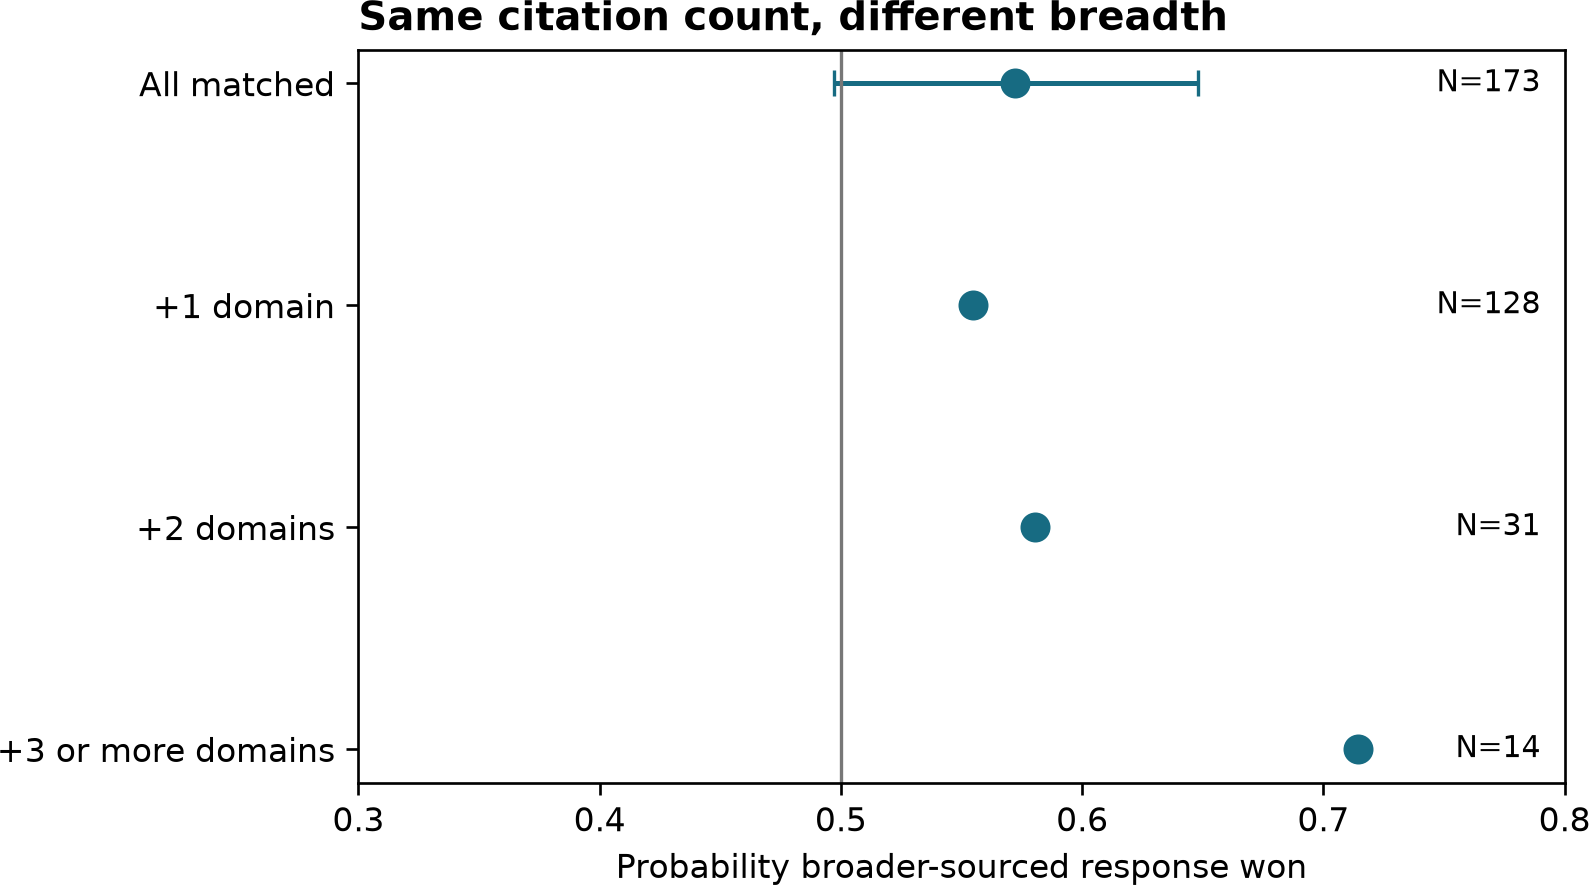
\includegraphics[width=0.90\textwidth]{figures/matched_analysis.png}
\caption{Exact citation-count comparison. Points show the probability that the broader-sourced response won. The ``All equal-count'' interval is the judge-cluster bootstrap 95\% CI; smaller strata are shown descriptively with their sample sizes. The vertical line marks 0.50; the descriptive binomial test for the all-equal-count estimate gives $p=.068$.}
\Description{Plot of broader-sourced response win probabilities among battles with equal citation counts. Overall probability is about 0.572 with a confidence interval crossing 0.50. Point estimates rise from roughly 0.555 for a one-domain advantage to 0.714 for an advantage of three or more domains, while sample sizes decrease.}
\label{fig:matched}
\end{figure*}

\subsection{RQ3: Intent heterogeneity}
The pre-specified, model-by-intent-adjusted omnibus interaction was significant, $LR(14)=27.05$, $p=.019$, on 4,108 battles with one of the eight pre-specified intent labels. However, no intent-specific redundancy coefficient survived Holm correction; the smallest adjusted $p$ was .189. We therefore do not interpret any individual intent coefficient as a finding. Because intent labels are released automated annotations, the omnibus result is treated only as secondary evidence that the pooled relationship may be nonuniform, not as evidence for any particular task-specific rule (Figure~\ref{fig:intent}).

\begin{figure*}[t]
\centering
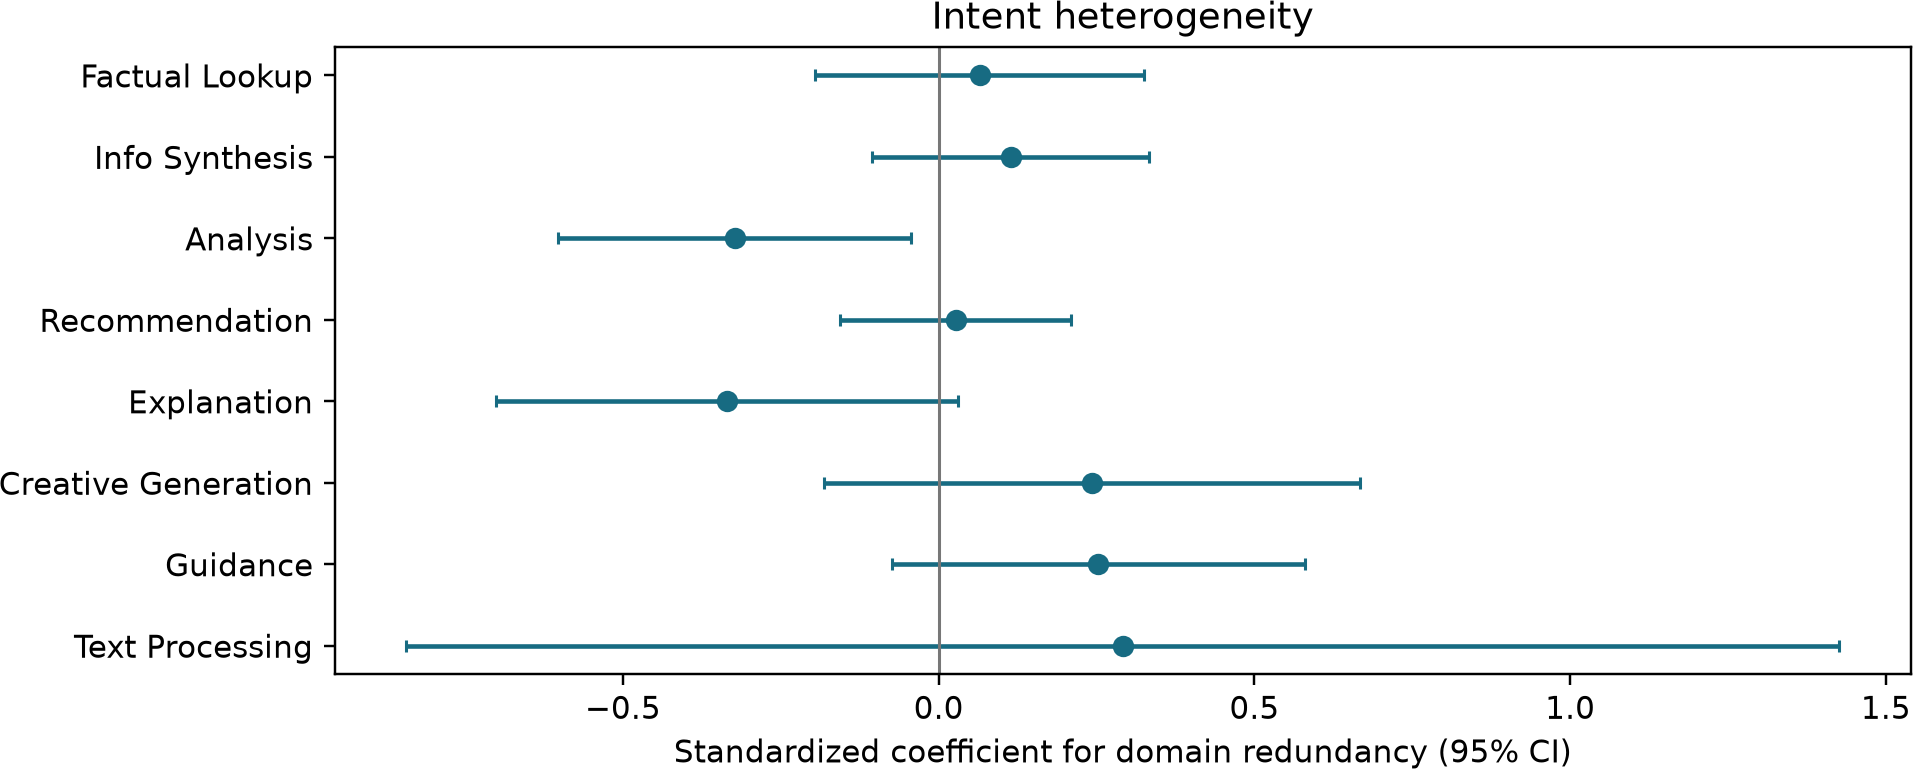
\includegraphics[width=0.92\textwidth]{figures/intent_heterogeneity.png}
\caption{Intent-specific standardized redundancy coefficients with 95\% confidence intervals ($N=4{,}108$). The omnibus interaction is significant, but no individual intent survives Holm correction. Negative coefficients correspond to greater domain breadth being associated with preference at fixed citation quantity.}
\Description{Forest plot for eight intent categories. Estimates vary across positive and negative values. Analysis and Explanation are negative; several other intents are positive. Most confidence intervals cross zero, and the small Text Processing group has a very wide interval.}
\label{fig:intent}
\end{figure*}

\subsection{Robustness and model-pair heterogeneity}
Most full-sample sensitivity analyses remained close to zero. The redundancy coefficient was 0.022 using all languages, 0.005 using all turns, 0.032 with query-stripped URL identity, 0.002 using trace-grounded citations only, 0.007 under conservative bare-URL handling, 0.012 among complete numeric-marker resolutions, and $-0.018$ after omitting source-category controls. Restricting to battles where both responses used Arena's standardized citation format gave $\beta=-0.111$ (95\% CI $[-0.354,0.132]$, $N=929$), while a tie-inclusive sensitivity gave $\beta=0.020$ (95\% CI $[-0.052,0.092]$, $N=6{,}162$). Model-by-calendar-week and model-by-client-country nuisance interactions produced coefficients of 0.030 and 0.032, respectively. Giving each judge equal total weight yielded $\beta=-0.001$ with a bootstrap interval spanning zero. Alternative breadth measures likewise had intervals crossing zero; their coefficient signs are not directly comparable with redundancy because larger values represent broader sourcing.

Exact model-pair analyses were less uniform. Of five qualifying pairs, two had intervals excluding zero in opposite directions: gpt-4o-search-high-loc versus sonar-reasoning-pro-high produced a positive redundancy estimate ($\beta=1.073$, 95\% CI [0.090, 2.056]), whereas gpt-4o-search-high versus sonar-reasoning produced a negative estimate ($\beta=-1.092$, 95\% CI $[-1.905,-0.279]$). One other pair was near zero, and two pair-specific fits had unstable standard errors. These pair-specific estimates are diagnostic transportability checks rather than multiplicity-adjusted discoveries; we use their opposite directions as evidence of instability, not as standalone confirmatory effects. This sign disagreement argues against interpreting the pooled coefficient as a model-independent behavioral law (Figure~\ref{fig:robustness}).

\begin{figure*}[t]
\centering
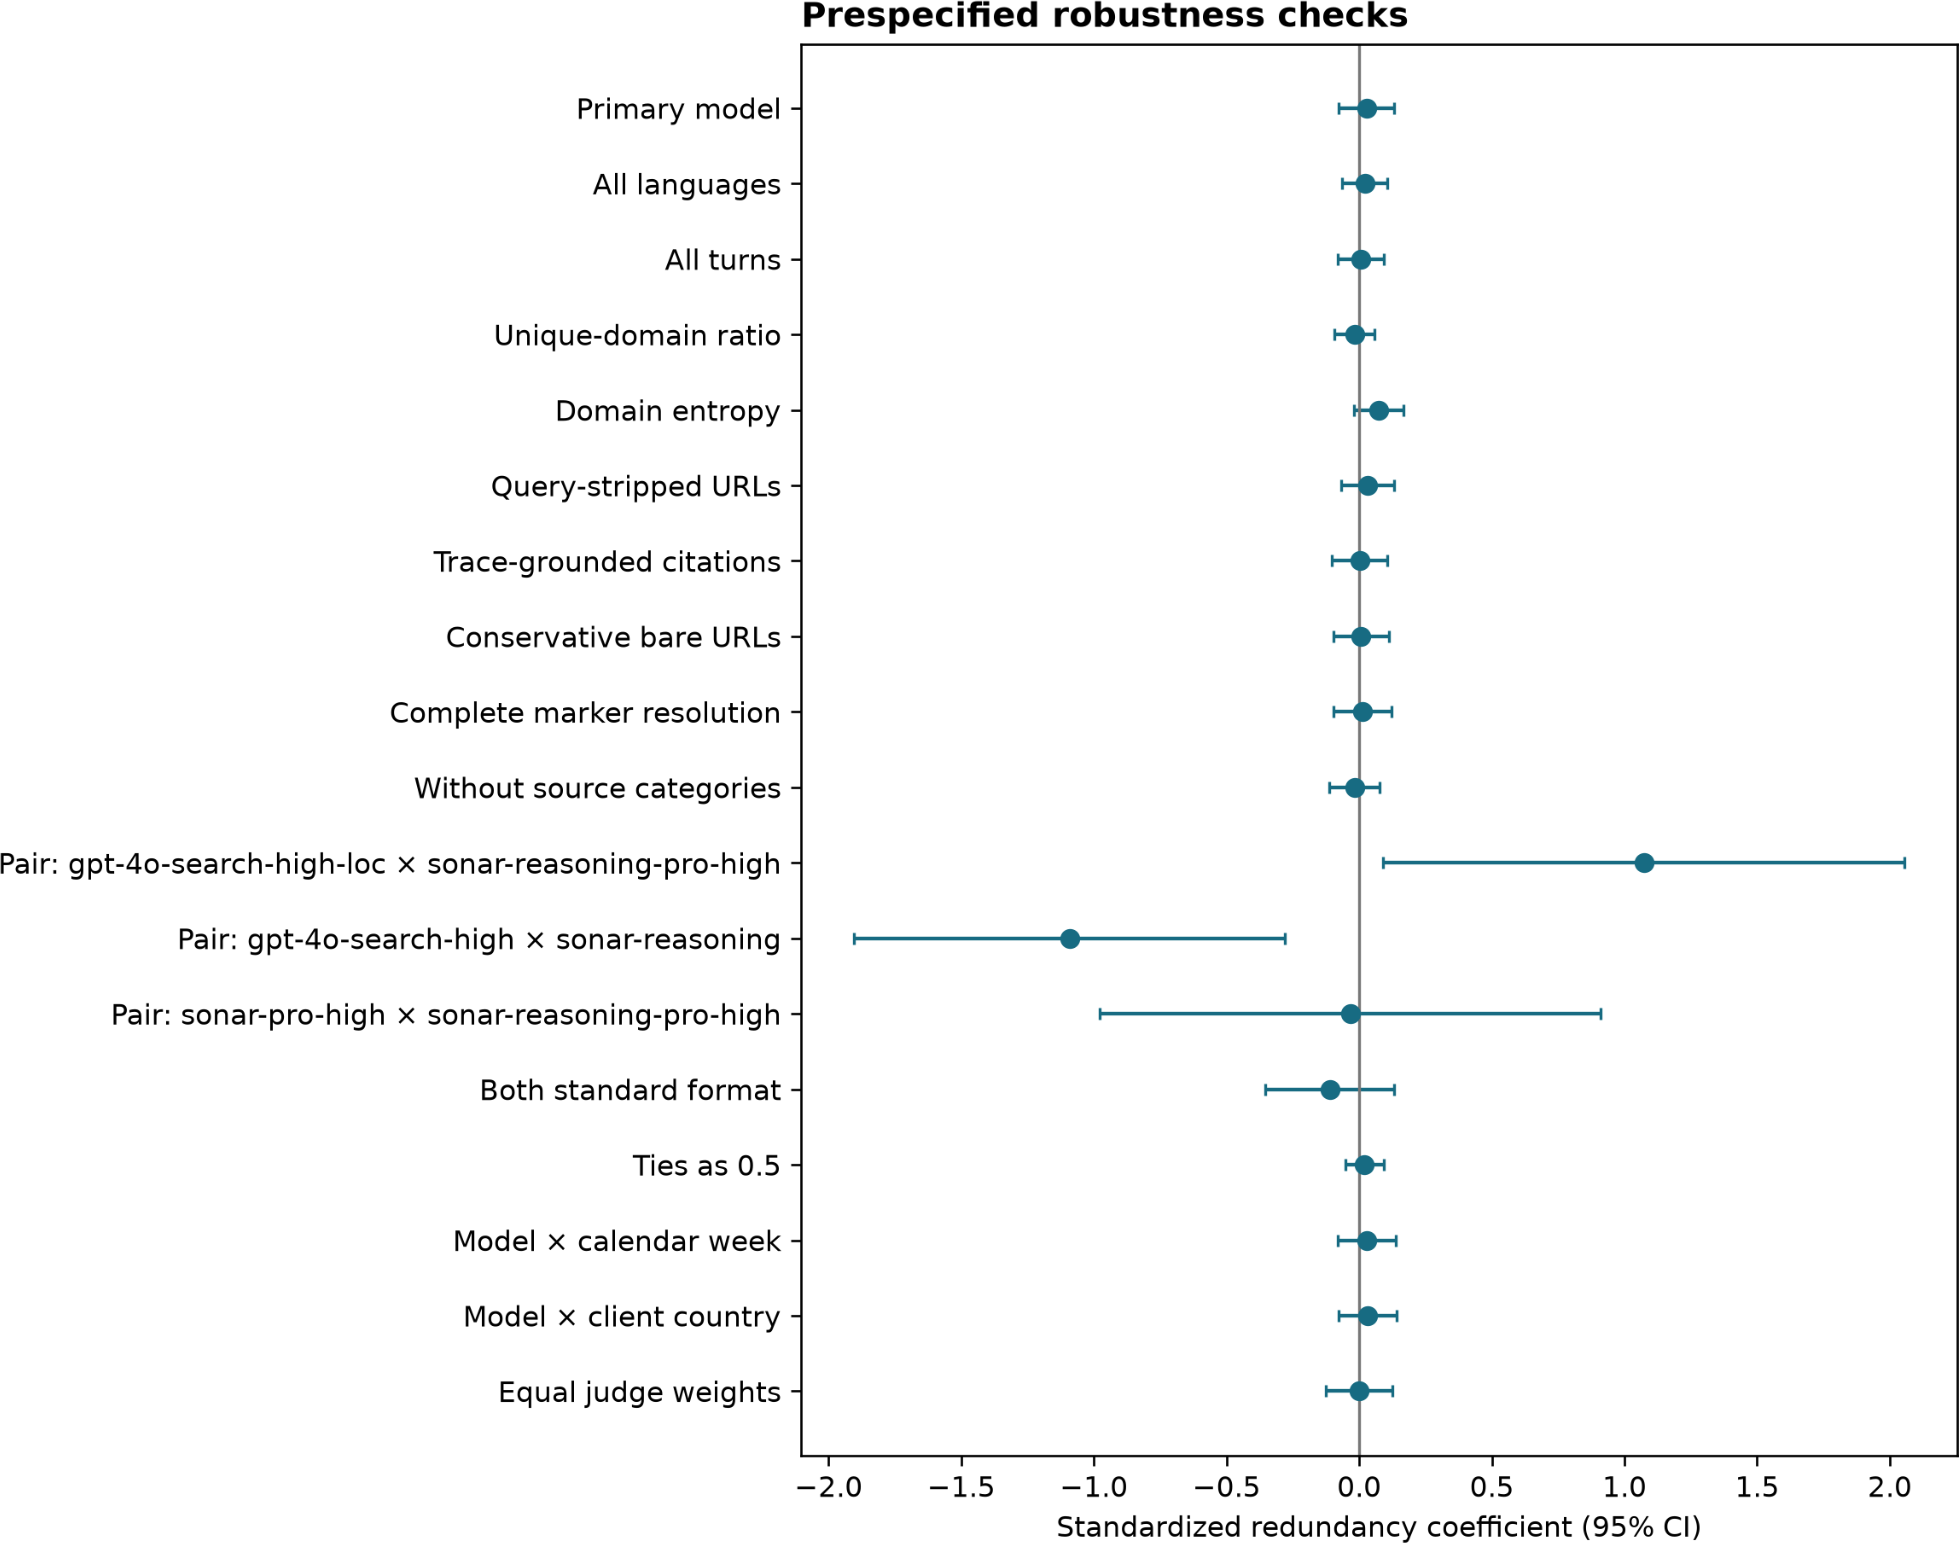
\includegraphics[width=0.94\textwidth]{figures/robustness_forest.png}
\caption{Pre-specified robustness checks. Full-sample sensitivities cluster near zero. Exact model-pair estimates are more heterogeneous, including two intervals excluding zero in opposite directions; unstable pair-specific fits are shown only as point estimates where uncertainty was not interpretable.}
\Description{Large forest plot of robustness estimates. Most rows lie close to zero with intervals crossing zero. Two exact model-pair rows are far from zero in opposite directions, one positive near 1.07 and one negative near -1.09, while other robustness checks remain close to zero.}
\label{fig:robustness}
\end{figure*}

The planned citation-attribution-quality sensitivity could not be computed because the public parquet used for this run does not contain the Support/Irrelevant/Contradict attribution labels required by the frozen specification. We did not create replacement labels or introduce new LLM judging after outcome inspection.

\section{Discussion}
\subsection{What the pooled result establishes}
Across the frozen primary model, practical-effect calculations, and held-out validation, we do not find a clearly estimated \emph{overall} association between registrable-domain breadth and human preference once citation quantity and the other measured controls are included. This is not evidence that source breadth never matters, nor is it a formal equivalence result. The primary interval still permits modest effects in either direction, and the exact-count comparison leans somewhat toward broader sourcing. The defensible conclusion is narrower: breadth does not behave as a stable, general preference cue in this Search Arena sample in the way citation quantity and response length do.

That distinction is substantively important. The positive citation-quantity control replicates prior evidence that users tend to prefer responses with more citations, but distributing those citations across more domains contributes essentially no overall incremental fit or out-of-sample prediction in our specification. Thus, if an evaluation already rewards citation count, adding unique-domain count as an additional ``richness'' bonus encodes a second user-preference assumption that is not supported here. Our evidence supports reporting breadth as a transparent exposure descriptor; it does not support a generic positive preference bonus for breadth; and it does not test whether breadth is valuable for different objectives such as coverage or verification. Evaluations that collapse abundance and breadth into one score may therefore hide different relationships with human judgment.

\subsection{Why the near-zero result is informative}
A near-zero novel coefficient is only useful if it is distinguishable from a failed measurement pipeline. Three features of the analysis reduce that concern. First, the same reconstructed features recover the previously reported positive directions for response length and citation quantity. Those positive controls establish sensitivity to known preference correlates; they do \emph{not} by themselves validate registrable-domain breadth as a proxy for diversity, quality, or independent evidence, which is precisely the construct question at issue. Second, the primary sample contains substantial within-battle redundancy variation, the design is full rank and well conditioned, and visible-reference parsing is high across major model families. Third, the conclusion is stable across alternative URL rules, trace-grounded citations, marker-resolution restrictions, language, conversation depth, time, locale, and judge weighting. These checks do not prove perfect measurement, but they make a simple ``the parser could not detect preference signals'' explanation less plausible.

The absence of held-out improvement is equally important. A feature can be statistically interpretable yet still add no practical information for ranking or evaluation. Here the breadth term neither improves average fit nor predicts unseen judge-grouped battles more reliably, while exact model-pair estimates disagree in sign. Read through the validation lens in Table~\ref{tab:validity}, breadth passes the first hurdle---it is a measurable source-structure construct separable from citation count---but receives little support for incremental preference validity and limited support for transportability. That pattern is more informative than a binary significant/non-significant label: it distinguishes a useful descriptor of information exposure from a general-purpose preference metric.

\subsection{Breadth appears context-dependent rather than universally beneficial}
The exact-count estimate cautions against reading the pooled near-zero coefficient as proof of irrelevance: among equal citation counts, broader-sourced answers won 57.2\% of comparisons, but with an interval that includes 50\%. Because the exact-count subset and full-sample model target different estimands, the difference in point estimates is not itself evidence of contradiction. The two results are compatible if any breadth effect is modest, concentrated in the exact-count subset, context-dependent, or partly averaged away by system-specific behavior.

The heterogeneity analyses reinforce that interpretation. The omnibus intent interaction indicates that citation-feature relationships are not perfectly constant across tasks, but no individual intent survives multiplicity correction. More strikingly, exact model-pair estimates point in opposite directions for two qualifying pairs. One plausible explanation is that breadth interacts with model-specific retrieval, writing, or citation behavior rather than operating as an independent universal signal. Another is residual observational confounding: even within exact model pairs, source structure may correlate with unmeasured answer qualities. The present design can reveal instability but cannot identify its mechanism.

These patterns fit broader CHIIR evidence that information-seeking outcomes depend not only on what information is available but on how interfaces direct attention, trust, verification, and effort \citep{mayerhofer2025blending,bink2026canyoutellme,he2026transparency}. If users rarely inspect sources, breadth may function only weakly as a visible cue; if they do inspect, its value may depend on the task, the perceived authority of domains, and the surrounding interface.

\subsection{Implications for generative-search evaluation and design}
\paragraph{Separate abundance from breadth.}
Citation quantity, domain breadth, source type, and citation quality should be reported as distinct dimensions. A system can surface many links from few domains or fewer links from many domains, and these configurations need not receive the same preference response. Benchmarks should avoid treating unique-domain count as a drop-in substitute for citation count or combining them into an opaque composite without a clear user-centered rationale.

\paragraph{Do not optimize mechanically for more domains.}
Our results do not justify rewarding systems simply for increasing registrable-domain count. Broader sourcing can be useful for coverage or verification, but it may also trade off against topical authority, coherence, or inspection effort. If a system is designed to expose multiple sources, interface support should help users understand and compare those sources rather than assuming that diversity is self-explanatory. This is especially relevant given evidence that presentation changes source attention while clicks remain sparse \citep{he2026transparency}.

\paragraph{Retain task- and model-level diagnostics.}
A single pooled coefficient can hide meaningful differences across model pairs and information needs. Evaluations of generative search should therefore report transportability checks across major systems and tasks, particularly when a metric is proposed as a general-purpose ranking or quality signal.

\paragraph{Treat predictive value as part of metric validation.}
If a feature is proposed as a useful evaluation signal, statistical association alone is not enough; it should ideally improve decisions or prediction on held-out data. Here, adding redundancy changed neither log loss nor Brier score in a practically meaningful way. Following established metric-validity principles rather than proposing a new universal framework, we use construct separation, incremental fit/prediction, and transportability as checks on this concrete candidate metric. Within this dataset and these controls, domain breadth is better viewed as a descriptive property of information exposure than as a reliable standalone predictor of preference.

\subsection{Values and construct boundaries}
Metric choice is also a values choice. Treating ``more domains'' as inherently better would encode an untested preference for breadth that our data do not support, while registrable-domain count does not itself measure viewpoint diversity, evidential independence, authority, or truth. Designers and evaluators should state which property they value---coverage, verification opportunity, perspective diversity, source independence, or something else---and measure that construct as directly as possible. Domain breadth is useful as a transparent description of visible exposure; it should not silently stand in for broader normative goals.

\section{Limitations}
\paragraph{Construct validity.}
Registrable-domain breadth is deliberately narrower than source diversity in a normative sense. Different domains may share ownership, syndicate the same reporting, rely on common upstream evidence, or represent similar viewpoints. We therefore do not interpret $U$ as viewpoint diversity, evidential independence, or factual quality.

\paragraph{Causal identification.}
Search Arena contains naturally occurring pairwise preferences rather than randomized manipulation of source breadth. The primary model, exact-count comparison, source-category controls, model-pair analyses, and time/locale sensitivities reduce specific alternative explanations but cannot establish that changing domain breadth would causally change preference. The exact-count subset fixes citation quantity only; it is not propensity matching or a causal design. Unobserved response qualities may influence both sourcing structure and human judgments.

\paragraph{Attention and mechanism.}
Preference logs do not reveal whether judges opened citations, noticed source domains, or consciously used sourcing structure when deciding. We therefore estimate an answer-level association, not a cognitive mechanism. That absence limits mechanistic claims but does not change the narrower evaluative question of whether breadth adds information about preference.

\paragraph{Dependence structure.}
Judge clustering captures repeated observations from the same released judge identifier, and the first-turn restriction removes repeated turns within a conversation. The release does not provide a validated semantic query-family identifier, however, so semantically similar prompts from different judges are treated as separate stimuli. If such prompt families induce residual correlation, the reported uncertainty could be understated.

\paragraph{Telemetry and measurement.}
Provider search traces can be incomplete and citation formats differ across systems. Our primary construct is therefore based on user-visible citations, with numeric markers resolved through disclosed traces and direct visible URLs measured independently of backend telemetry. High resolution coverage does not guarantee semantic correctness of every parsed source, and we do not manually validate every citation. Format-restricted, trace-grounded, conservative-URL, and complete-resolution sensitivities reduce this concern, but unobserved retrieval behavior cannot be reconstructed.

\paragraph{External validity.}
Search Arena users are self-selected, the observations reflect specific model versions and deployment periods, and the primary analysis is English and first-turn by design. All-language and all-turn analyses probe some boundaries, but results should not be generalized automatically to all search users, languages, future systems, or interface designs. Released intent annotations are automated and therefore support only secondary heterogeneity analysis.

\paragraph{Sparse subgroup estimates.}
The exact citation-count comparison contains only 173 breadth-different battles, and the larger breadth-advantage strata are especially small. Its 95\% interval includes 50\%, so the 57.2\% point estimate is descriptive rather than confirmatory. Exact model-pair analyses likewise become noisy quickly, with two qualifying fits showing unstable standard errors. These limitations make small or highly localized breadth effects difficult to resolve.

\paragraph{Functional form.}
The primary model estimates a single additive linear effect of standardized redundancy on the log-odds of preference. A genuinely nonlinear or thresholded relationship could therefore average toward zero. The pre-specified ratio/entropy alternatives and exact-count strata probe related structure, but the sparse larger-breadth strata do not support a reliable dose-response claim.

\paragraph{Unavailable attribution labels.}
The frozen plan included a citation-attribution-quality sensitivity using Search Arena's released Support/Irrelevant/Contradict labels. Those labels are distributed in a separate released attribution subset and are not present in the frozen feature parquet used for this analysis. Merging a new derived file after inspecting the primary outcome would have changed the frozen data lineage; we therefore report this pre-specified sensitivity as unavailable rather than construct a post-outcome join or create new annotations.

\section{Conclusion}
Using 4,265 decisive, English, first-turn Search Arena battles and an outcome-blind frozen analysis, we separated citation quantity from registrable-domain breadth in user-visible generative-search responses. Citation quantity and response length reproduced positive preference associations, but same-domain redundancy showed no clearly estimated overall association after the pre-specified controls ($\beta=0.028$, bootstrap 95\% CI $[-0.071,0.127]$) and no reliable held-out predictive gain. A smaller exact-count comparison leaned toward broader sourcing, while intent and exact model-pair analyses indicated heterogeneity without a stable intent-specific effect. The main lesson is therefore not that breadth is irrelevant, but that measurability does not guarantee preference validity: breadth is not interchangeable with citation abundance and does not behave as a portable preference signal in this dataset. The contribution is an empirical boundary condition for preference-oriented generative-search evaluation, not a new general metric theory: adjacent source features computed from the same citation set need not share user-centered validity. Future work should manipulate citation count and breadth independently in randomized retrieval or interface experiments, measure whether users actually inspect and compare sources, and test outcomes such as factual verification, calibrated trust, and knowledge gain in addition to preference.

\bibliographystyle{ACM-Reference-Format}
\bibliography{references}

\end{document}
